\chapter{Quasinormal Modes}
\label{ch:qnm}

\begin{chapterlead}
When a photonic resonator is open to its environment, its ``modes'' are
not the orthogonal, real-frequency eigenstates of Hermitian spectral
theory. They are \emph{quasinormal modes}: solutions of the source-free
Maxwell equations with outgoing boundary conditions, possessing complex
eigenfrequencies and field profiles that diverge at spatial infinity.
Quasinormal modes are derived from the Maxwell operator. Their
normalization and inner product differ from those of closed cavities,
and they describe open photonic systems ranging from nanophotonic
cavities to diffraction gratings.
\end{chapterlead}


%% ================================================================
\section{Defining quasinormal modes}
\label{sec:qnm-definition}

A \emph{quasinormal mode} (QNM) of an open electromagnetic system is a
solution to the source-free vector Helmholtz equation
\begin{equation}
 \curl\!\left[\frac{1}{\epsr(\rr)}\,\curl\tilde{\HH}_n(\rr)\right]
 = \frac{\omtil_n^2}{c^2}\,\tilde{\HH}_n(\rr),
 \label{eq:qnm-evp}
\end{equation}
subject to the \emph{outgoing-wave} (Silver--M\"uller) boundary condition
introduced in Section~\ref{sec:outgoing-bc}. The tilde distinguishes QNM
fields and frequencies from their Hermitian counterparts.

Because the boundary condition is frequency-dependent, the problem is
nonlinear in $\omtil$: we seek pairs $(\omtil_n, \tilde{\HH}_n)$
simultaneously. For a passive system without gain, all QNM frequencies
lie in the lower half of the complex $\omega$ plane:
\begin{equation}
 \omtil_n = \omega_n - i\gamma_n, \qquad \gamma_n > 0,
 \label{eq:qnm-freq}
\end{equation}
where $\omega_n$ is the resonant frequency and $\gamma_n$ the radiative
decay rate. The quality factor is $\Qfac_n = \omega_n/(2\gamma_n)$.

As established in Section~\ref{sec:poles-zeros-ch4}, the QNM frequencies
coincide with the poles of the scattering matrix $\Smat(\omega)$: at
$\omega = \omtil_n$, an outgoing field exists with no incoming excitation.

\subsection{Example: Fabry--P\'erot QNMs}
\label{ssec:qnm-fabry-perot}

The simplest system with QNMs is a dielectric slab of thickness $L$ and
real refractive index $n$ in vacuum. The QNM condition requires outgoing
waves on both sides, which is equivalent to the round-trip resonance
condition with the Fresnel reflection coefficient
$r = (n-1)/(n+1)$:
\begin{equation}
 r^2 e^{2in\omtil L/c} = 1.
 \label{eq:fp-qnm-condition}
\end{equation}
Solving for $\omtil$ gives the QNM frequencies
\begin{equation}
 \omtil_m = \frac{c}{nL}\left(m\pi - \arg r\right)
 - i\,\frac{c}{nL}\ln\frac{1}{|r|},
 \qquad m = 0, \pm 1, \pm 2, \ldots
 \label{eq:fp-qnm-freqs}
\end{equation}
All frequencies have the same imaginary part
$\gamma = (c/nL)\ln(1/|r|)$, set by the mirror reflectivity. For a
silicon slab ($n = 3.5$, $L = 300\;\mathrm{nm}$):
\begin{itemize}
 \item $|r| = (3.5-1)/(3.5+1) = 0.556$, so $\ln(1/|r|) = 0.588$.
 \item $\gamma = c \times 0.588 / (3.5 \times 300\;\mathrm{nm})
 \approx 1.68 \times 10^{14}\;\mathrm{rad/s}$.
 \item $\Qfac \approx \omega_0/(2\gamma)$. For the fundamental mode
 at $\lambda \approx 2nL = 2100\;\mathrm{nm}$
 ($\omega_0 \approx 8.97 \times 10^{14}\;\mathrm{rad/s}$),
 $\Qfac \approx 2.7$.
\end{itemize}
This very low $\Qfac$ reflects the poor confinement of a bare slab.
Adding distributed Bragg reflectors raises $|r|$ and pushes the QNM
poles closer to the real axis.

\paragraph{QNM field profile inside and outside the slab.}
Inside the slab ($0 < z < L$), the QNM field is a standing wave:
$\tilde{E}_m(z) \propto \sin(n\omtil_m z/c)$ (for the $\EE$-field of a
TE mode at normal incidence). Outside the slab ($z > L$ or $z < 0$),
the field has the outgoing-wave form
$\tilde{E}_m(z) \propto e^{+i\omtil_m z/c}$ for $z > L$ and
$e^{-i\omtil_m z/c}$ for $z < 0$. Writing
$\omtil_m = \omega_m - i\gamma$, the far-field amplitude is
$|\tilde{E}_m(z)| \propto e^{\gamma|z|/c}$: the field grows
exponentially away from the slab, as derived in
Section~\ref{sec:qnm-divergence}. At a distance of
$z = c/\gamma \approx 1.78\;\mu$m (for the silicon slab above), the
field amplitude has grown by a factor of $e \approx 2.72$.
At $z = 10\;\mu$m, it has grown by a factor of $e^{5.6} \approx 270$.
This rapid spatial growth is what makes the standard $L^2$ norm diverge
and necessitates the unconjugated normalization of
Section~\ref{sec:qnm-normalization}.

\begin{figure}[t]
 \centering
 
\includegraphics[width=0.92\textwidth]{fig_f6_fabry_perot_qnm.pdf}
 \caption{Quasinormal-mode poles of a one-dimensional Fabry--P\'erot resonator. Panel (a) plots the pole positions from the round-trip condition $r^2\exp(2in\tilde{\omega}L/c)=1$ for several mirror reflectivities; the compact legend identifies the $|r|$ value for each pole row, and the in-panel formula gives the imaginary part $\mathrm{Im}\,\tilde{\omega}=-c\ln(1/|r|)/(nL)$. Increasing $|r|$ moves the pole rows upward toward the real-frequency axis while remaining in the passive lower half-plane. Panel (b) shows the fundamental quality factor $Q=\mathrm{Re}\,\tilde{\omega}_1/(2|\mathrm{Im}\,\tilde{\omega}_1|)$ as a function of amplitude reflectivity, with colored markers corresponding to the same $|r|$ values as the pole rows. The gray marker denotes the bare silicon--air interface example used in the text, with $n=3.5$, $L=300\,\mathrm{nm}$, $|r|=0.556$, and $Q\approx2.67$.}
 \label{fig:fabry-perot-qnm-poles}
\end{figure}


%% ================================================================
\section{Spatial divergence and its physical meaning}
\label{sec:qnm-divergence}

A QNM with complex frequency $\omtil_n = \omega_n - i\gamma_n$ has far-field
spatial behavior
\begin{equation}
 \tilde{\HH}_n(\rr) \;\sim\;
 \frac{e^{i\omtil_n r/c}}{r}\,\mathbf{f}_n(\hat{\rr})
 = \frac{e^{i\omega_n r/c}\,e^{\gamma_n r/c}}{r}\,\mathbf{f}_n(\hat{\rr}),
 \label{eq:qnm-farfield}
\end{equation}
where $\mathbf{f}_n$ is an angular pattern. The factor $e^{\gamma_n r/c}$
\emph{grows} exponentially with distance. This is deeply
counterintuitive---how can a decaying mode grow in space?

The resolution is causal: the QNM represents a field pattern that was
established at some time in the past and has been radiating ever since.
At a distant point $r$, we observe light that was emitted at the earlier
time $t - r/c$, when the mode had amplitude $e^{-\gamma_n(t - r/c)}$.
The product of the temporal decay and the retardation gives
$e^{-\gamma_n t}\,e^{\gamma_n r/c}$: at fixed $t$, the field grows with
$r$ because distant points sample the mode at earlier, stronger times.

This exponential growth means that the standard $L^2$ norm
$\int|\tilde{\HH}_n|^2\;\dd^3 r$ diverges. The QNM is \emph{not
square-integrable} and cannot be normalized with the Hermitian inner
product of Chapter~\ref{ch:energy-inner}. A different normalization
scheme is needed.

\begin{figure}[t]
 \centering
 
\includegraphics[width=0.92\linewidth]{fig_f6_qnm_divergence.pdf}
 \caption{Field envelope $|\tilde{E}(z)|$ of the fundamental
 quasinormal mode of a dielectric slab ($n = 3.5$,
 $L = 300\;\mathrm{nm}$) in vacuum, normalized to the slab-interior
 maximum. The mode is the symmetric
 $\cos\tilde{k}(z - L/2)$ solution. Outside the slab, the
 outgoing-wave boundary condition produces exponential growth
 $\propto e^{\gamma|z|/c}$ on both sides, where
 $\gamma = -c\ln|r|/(nL)$ is the radiative decay rate from
 Eq.~\eqref{eq:qnm-freq}. This divergence is the defining feature
 of QNMs and is regularized by perfectly matched layers
 (Section~\ref{sec:qnm-pml}). Shaded region marks the slab.}
 \label{fig:qnm-field-divergence}
\end{figure}

\subsection{Connection to the skin effect}
\label{ssec:divergence-skin}

The spatial divergence of a single QNM has a close analogy with the
non-Hermitian skin effect (Chapter~\ref{ch:skin-effect}): in both cases,
the non-Hermitian boundary condition forces eigenstates to have
exponentially growing or decaying spatial profiles rather than the
oscillatory behavior of Hermitian modes. The QNM divergence is the
single-resonator version of a phenomenon that, in periodic systems,
becomes the collective skin effect.

%% ================================================================
\section{PML regularization and the non-self-adjoint operator}
\label{sec:qnm-pml}

The perfectly matched layers introduced in Section~\ref{sec:pml} provide
both a computational tool and a conceptual resolution of the divergence
problem. By applying a complex coordinate stretching $\rr \to \tilde{\rr}$
in the absorbing layer, the PML maps the outgoing-wave problem on an
infinite domain to an eigenvalue problem on a bounded domain with a
\emph{non-self-adjoint} operator~\cite{vial2014quasimodal}.

\subsection{How PML regularization works}
\label{ssec:pml-mechanism}

In the PML-regularized problem:
\begin{enumerate}
 \item The QNM fields are damped in the PML region and become
 square-integrable on the computational domain.
 \item The true QNM eigenfrequencies $\omtil_n$ (poles of $\Smat$) are
 unchanged---they are intrinsic to the scatterer and independent
 of the PML parameters.
 \item The continuous spectrum of radiation modes is discretized by the
 finite PML, producing a set of ``PML modes'' that depend on the
 PML thickness and absorption strength.
 \item The transformed Maxwell operator is non-self-adjoint: its
 eigenvectors are not orthogonal under the standard $L^2$ inner
 product.
\end{enumerate}

\subsection{PML validation and spurious modes}
\label{ssec:pml-validation}

The PML introduces two practical concerns:
\begin{itemize}
 \item \textbf{Spurious PML modes:} the discretized radiation continuum
 produces a set of modes whose eigenfrequencies depend on the PML
 parameters. These must be distinguished from the physical QNMs,
 whose eigenfrequencies converge as the PML thickness and absorption
 increase. A standard check is to vary the PML parameters and
 identify eigenfrequencies that remain stable.
 \item \textbf{PML thickness and absorption:} the PML must be thick
 enough and absorbing enough to suppress reflections from the outer
 boundary. For QNMs with large $\gamma_n$ (low $\Qfac$), the spatial
 growth rate $\gamma_n/c$ is large, and the PML must compensate this
 growth before the field reaches the outer boundary. A rule of thumb
 is that the PML absorption over its thickness should provide at least
 $20\;\mathrm{dB}$ of suppression.
\end{itemize}

The price of PML regularization is that the operator is now manifestly
non-Hermitian. The tools of Hermitian spectral theory do not apply.
Instead, we must use the \emph{adjoint} operator and \emph{biorthogonal}
relations.

\paragraph{PML convergence in practice~\cite{opg2023dispersive,v2024exact}.}
For the silicon Fabry--P\'erot slab ($n = 3.5$, $L = 300\;\mathrm{nm}$),
a PML of thickness $d_{\mathrm{PML}} = 2\lambda$ with a quadratic
absorption profile $\sigma(s) = \sigma_{\max}(s/d_{\mathrm{PML}})^2$
converges the fundamental QNM frequency to four significant figures once
$\sigma_{\max} \gtrsim 3\,\omega/c$. Beyond that value the pole
position is insensitive to PML parameters---the hallmark of a
well-converged QNM calculation, because the physical eigenfrequency is a
property of the resonator, not of the absorbing boundary. A useful
convergence diagnostic is the mode ratio
$\eta = |\tilde{E}_{\mathrm{PML,outer}}|/|\tilde{E}_{\max}|$: when
$\eta < 10^{-3}$, the field has decayed sufficiently within the PML and
the eigenvalue is converged to better than $0.1\%$. This criterion
translates into a minimum PML thickness of roughly $1.5$--$2$ wavelengths
for moderate-$\Qfac$ resonators ($\Qfac \sim 10$) and can be relaxed to
$\sim 1\lambda$ for high-$\Qfac$ modes ($\Qfac > 10^3$) whose
far-field divergence rate $\gamma/c$ is small.


%% ================================================================
\section{The adjoint problem and biorthogonality}
\label{sec:qnm-adjoint}

\subsection{The adjoint Maxwell operator}
\label{ssec:adjoint-operator}

For the PML-regularized Maxwell operator $\Mop_{\mathrm{PML}}$, the
adjoint operator $\Mop_{\mathrm{PML}}^\adj$ is defined by the condition
\begin{equation}
 \langle\mathbf{F},\,\Mop_{\mathrm{PML}}\mathbf{G}\rangle
 = \langle\Mop_{\mathrm{PML}}^\adj\mathbf{F},\,\mathbf{G}\rangle
 \label{eq:adjoint-def}
\end{equation}
for all fields in the domain. For a reciprocal medium (symmetric
$\epsr$ tensor), the adjoint operator takes a remarkably simple form:
its eigenvectors $\tilde{\HH}_n^{\mathrm{L}}$ satisfy the same
differential equation~\eqref{eq:qnm-evp} but with \emph{incoming-wave}
boundary conditions---the time-reverse of the QNM
problem~\cite{vial2014quasimodal}.

\subsection{Biorthogonality}
\label{ssec:biorthogonality}

The ``left'' (adjoint) eigenvectors $\tilde{\HH}_m^{\mathrm{L}}$ and
``right'' (direct) eigenvectors $\tilde{\HH}_n$ satisfy a biorthogonality
relation:
\begin{equation}
 \bigl\langle\tilde{\HH}_m^{\mathrm{L}},\,
 \tilde{\HH}_n\bigr\rangle_{\mathrm{PML}}
 = \delta_{mn},
 \label{eq:biorthogonality}
\end{equation}
after appropriate normalization. This is the non-Hermitian analogue of
mode orthogonality. The subscript PML indicates that the integral is over
the computational domain including the PML region.

\subsection{Physical interpretation}
\label{ssec:biorthogonal-physics}

The biorthogonality relation has a direct physical interpretation:
$\langle\tilde{\HH}_m^{\mathrm{L}}|\tilde{\HH}_n\rangle = 0$ for
$m \neq n$ means that the \emph{time-reversed} field of mode $m$
has zero overlap with the forward field of mode $n$. This is a
statement about reciprocity: the mode $m$ launched backward does not
excite mode $n$ launched forward. This reciprocal orthogonality replaces
the power orthogonality of Hermitian modes.

\begin{booknote}[Biorthogonality replaces orthogonality]
In Hermitian systems, left and right eigenvectors are simply complex
conjugates of each other, and the biorthogonality
relation~\eqref{eq:biorthogonality} reduces to ordinary orthogonality
$\langle\HH_m^*,\HH_n\rangle = \delta_{mn}$. In non-Hermitian systems,
left and right eigenvectors are generally different functions, and the
bilinear form $\langle\cdot,\cdot\rangle$ is not the same as the
Hermitian inner product $\langle\cdot|\cdot\rangle$.
\end{booknote}


%% ================================================================
\section{QNM normalization}
\label{sec:qnm-normalization}

The normalization of quasinormal modes is subtle because the standard
volume integral diverges. Several equivalent prescriptions exist.

\subsection{The unconjugated norm}
\label{ssec:unconjugated}

For a reciprocal system, the adjoint modes are related to the direct
modes by $\tilde{\HH}_n^{\mathrm{L}}(\rr) = \tilde{\HH}_n(\rr)$
(without complex conjugation), and the normalization condition
becomes~\cite{kristensen2011effective}
\begin{equation}
 \int_\Omega \epsr(\rr)\,\tilde{\EE}_n(\rr)\cdot\tilde{\EE}_n(\rr)
 \;\dd^3 r
 + \text{surface correction}
 = 1.
 \label{eq:unconjugated-norm}
\end{equation}
The crucial feature is that $\tilde{\EE}_n$ appears \emph{twice without
conjugation}: this is an unconjugated bilinear form, not a Hermitian
inner product. The ``norm'' is complex, and the ``mode volume'' derived
from it is also complex:
\begin{equation}
 \tilde{V}_n = \frac{1}{\epsr(\rr_0)\,\tilde{\EE}_n(\rr_0)\cdot
 \tilde{\EE}_n(\rr_0)},
 \label{eq:complex-mode-volume}
\end{equation}
evaluated at a point of interest $\rr_0$ (typically the field maximum).

\subsection{The surface-integral correction}
\label{ssec:surface-correction}

The unconjugated volume integral in~\eqref{eq:unconjugated-norm} still
diverges over infinite space. The PML regularization truncates the domain,
but in formulations without a PML one can add an analytic surface term
that cancels the far-field divergence~\cite{kristensen2011effective}.
For a nondispersive homogeneous exterior the correction has the schematic
form
\begin{equation}
 N_n =
 \int_{\Omega_R}
 \left[
 \epsr\,\tilde{\EE}_n\cdot\tilde{\EE}_n
 - \mur\,\tilde{\HH}_n\cdot\tilde{\HH}_n
 \right]\dd^3 r
 + S_R[\tilde{\EE}_n,\tilde{\HH}_n],
 \label{eq:surface-norm}
\end{equation}
where $\Omega_R$ is a finite volume bounded by a surface of radius $R$
and $S_R$ is an outgoing-wave surface functional determined by the
far-field expansion. Its role is not to add stored energy at the boundary,
but to analytically continue the divergent volume integral to a finite,
normalization-independent value. In modern computations this same
regularization is often achieved more cleanly by integrating the
unconjugated product over a PML-stretched domain.

\subsection{Comparison of normalization schemes}
\label{ssec:norm-comparison}

Three normalization schemes are commonly used in the literature:
\begin{enumerate}
 \item \textbf{PML-based:} integrate the unconjugated product over
 the PML domain. Simplest computationally but depends weakly on
 PML parameters.
 \item \textbf{Surface-corrected:} add the surface integral
 correction~\eqref{eq:surface-norm}. PML-independent to
 exponential accuracy.
 \item \textbf{Pole residue:} extract the normalization from the
 residue of the Green function at the QNM pole. Mathematically
 elegant and manifestly PML-independent, but requires a scattering
 calculation at complex frequency.
\end{enumerate}
All three give the same result when properly implemented. The choice is
a matter of computational convenience.

\subsection{The Petermann factor from the unconjugated norm}
\label{ssec:petermann-from-norm}

The complex mode volume~\eqref{eq:complex-mode-volume} has an imaginary
part that vanishes only when the mode is Hermitian. The ratio of the
Hermitian (conjugated) norm to the unconjugated norm defines the
\emph{Petermann factor}:
\begin{equation}
 K_n = \frac{\displaystyle\int |\tilde{\EE}_n(\rr)|^2\;\dd^3 r}
 {\displaystyle\left|\int
 \tilde{\EE}_n(\rr)\cdot\tilde{\EE}_n(\rr)\;\dd^3 r
 \right|},
 \label{eq:petermann-definition}
\end{equation}
where the numerator uses the conventional conjugated inner product and
the denominator is the absolute value of the unconjugated norm. By the
Cauchy--Schwarz inequality, $K_n \ge 1$, with equality if and only if
$\tilde{\EE}_n$ can be chosen everywhere real---i.e.\ the mode is
Hermitian.

To see why $K_n$ measures excess noise and non-orthogonality, note that
the biorthogonal overlap of mode $n$ with its adjoint partner is
\begin{equation}
 \langle \tilde{\EE}_n^{\mathrm{L}} | \tilde{\EE}_n \rangle
 = \frac{1}{\sqrt{K_n}},
 \label{eq:petermann-phase-rigidity}
\end{equation}
so the \emph{phase rigidity} $r_n = K_n^{-1/2}$ measures how close
the right eigenvector is to the left eigenvector. At an exceptional
point, $\tilde{\EE}_n^{\mathrm{L}} \to \tilde{\EE}_m^{\mathrm{L}}$
(the two adjoint vectors coalesce), the overlap
$\langle \tilde{\EE}_n^{\mathrm{L}} | \tilde{\EE}_n \rangle \to 0$,
and $K_n \to \infty$.

The physical consequences of $K_n > 1$ are threefold. First, modal
non-orthogonality changes the residue of the Green tensor and therefore
the way spontaneous-emission noise and modal response are partitioned
among nearby resonances. In laser theory this is often summarized as a
Petermann enhancement of the effective modal noise. For an isolated mode
one often writes the scaling schematically as
\begin{equation}
 F_P \sim K_n\,\frac{3}{4\pi^2}\left(\frac{\lambda}{n}\right)^3
 \frac{Q}{V_{\mathrm{eff}}},
 \label{eq:purcell-petermann}
\end{equation}
where the precise prefactor depends on the QNM normalization, emitter
position, and the separation from neighboring modes. Second, the
fundamental linewidth of a laser operating on mode $n$ is
broadened by $K_n$ (the Schawlow--Townes linewidth multiplied by $K_n$),
because spontaneous emission into the non-orthogonal mode receives
contributions from all modes with nonzero overlap. Third, the
sensitivity of the eigenfrequency to perturbations scales as
$K_n^{1/2}$, connecting the Petermann factor to the enhanced sensing at
exceptional points discussed in Chapter~\ref{ch:exceptional-points}.

\paragraph{Example: plasmonic nanoparticle.}
For a silver nanoparticle of radius $a = 30\;$nm in air at the
localized surface plasmon resonance ($\lambda \approx 360\;$nm), the
mode volume is $|\tilde{V}| \approx 4 \times 10^{-5}\,\lambda^3$ and
the Petermann factor is $K \approx 1.3$---close to unity because the
mode is nearly Hermitian (low radiation loss). For a plasmonic dimer
with a $2\;$nm gap, the mode hybridization and near-field enhancement
push $K$ to $\sim 3$--$5$, and for coupled cavities tuned near an
exceptional point, $K$ can exceed $10^3$, dominating the noise budget.


%% ================================================================
\section{Modal expansion of the Green tensor}
\label{sec:green-tensor}

The electromagnetic Green tensor $\mathbf{G}(\rr,\rr';\omega)$ describes
the field at $\rr$ due to a point dipole source at $\rr'$. In the
spectral neighborhood of a QNM resonance $\omtil_n$, the Green tensor is
dominated by the QNM contribution:
\begin{equation}
 \mathbf{G}(\rr,\rr';\omega)
 \approx \sum_n
 \frac{c^2\,\tilde{\EE}_n(\rr)\otimes\tilde{\EE}_n(\rr')}
 {2\omtil_n(\omega - \omtil_n)},
 \label{eq:green-qnm}
\end{equation}
where the sum runs over QNMs near $\omega$ and the unconjugated
normalization~\eqref{eq:unconjugated-norm} has been used.

\subsection{Local density of states}
\label{ssec:ldos}

The local density of optical states (LDOS) at position $\rr$ is
proportional to the imaginary part of the Green tensor:
\begin{equation}
 \rho(\rr,\omega)
 = \frac{2\omega}{\pi c^2}\,\Im\!\bigl[\tr\mathbf{G}(\rr,\rr;\omega)\bigr].
 \label{eq:ldos}
\end{equation}
Near a QNM resonance, the LDOS exhibits an approximately Lorentzian peak
with width $2\gamma_n$ (where $\gamma_n = -\Im\omtil_n$ is the
half-width at half-maximum) and amplitude proportional to
$\Qfac_n/\Re\tilde{V}_n$.

\subsection{Purcell factor}
\label{ssec:purcell}

The Purcell factor---the enhancement of the spontaneous emission rate of
a quantum emitter at $\rr_0$ relative to free space~\cite{ren2021quasinormal,sauvan2014modal}---is the dipole-projected LDOS ratio
\begin{equation}
 F_P =
 \frac{\hat{\mathbf{d}}\cdot\Im\mathbf{G}(\rr_0,\rr_0;\omega)
 \cdot\hat{\mathbf{d}}}
 {\hat{\mathbf{d}}\cdot\Im\mathbf{G}^{(0)}(\rr_0,\rr_0;\omega)
 \cdot\hat{\mathbf{d}}},
 \label{eq:purcell-green}
\end{equation}
where $\hat{\mathbf{d}}$ is the dipole orientation and
$\mathbf{G}^{(0)}$ is the free-space Green tensor.  If $\mathbf{G}$ is
replaced by the scattered Green tensor, the equivalent form is
$F_P=1+\Gamma_{\mathrm{scatt}}/\Gamma_0$; Eq.~\eqref{eq:purcell-green}
uses the total Green tensor, so no extra background $1$ is added.  Near
an isolated QNM resonance with weak modal overlap, the QNM expansion~\eqref{eq:green-qnm} gives
\begin{equation}
 F_P \approx \frac{3}{4\pi^2}
 \left(\frac{\lambda_n}{n}\right)^{\!3}
 \frac{\Qfac_n}{\Re\tilde{V}_n},
 \label{eq:purcell-qnm}
\end{equation}
for emission near a single QNM resonance, where $\lambda_n$ is the
free-space wavelength, $n$ is the local refractive index, and
$\tilde{V}_n$ is expressed as a \emph{physical} volume (in units of
length${}^3$).  When the mode volume is instead quoted in units of
$\lambda^3$ or $(\lambda/n)^3$, the prefactor simplifies accordingly.

\paragraph{Numerical example: plasmonic nanocavity.}
For a gold nanoparticle dimer with a $2\;$nm gap in air, a full-wave
simulation gives $\omtil \approx (3.3 - 0.12i) \times 10^{15}\;$rad/s,
corresponding to $\lambda \approx 570\;$nm and
$\Qfac = \Re\omtil/(2|\Im\omtil|) = 3.3/(2 \times 0.12) \approx 13.8$.
The complex mode volume is
$\tilde{V} \approx (3.1 - 1.8i) \times 10^{-7}\,\lambda^3$, so
$\Re\tilde{V} \approx 3.1 \times 10^{-7}\,\lambda^3$. The resulting
Purcell factor at the gap centre is
\begin{equation}
 F_P \approx \frac{3}{4\pi^2}
 \frac{13.8}{3.1\times 10^{-7}}
 \approx 3.4 \times 10^6,
 \label{eq:purcell-plasmonic}
\end{equation}
where $n=1$ in the air gap and the mode volume is quoted in units of
$\lambda^3$, so the factor $(\lambda/n)^3$ in
Eq.~\eqref{eq:purcell-qnm} cancels the $\lambda^3$ denominator.
This enormous enhancement is a direct consequence of the extreme field
confinement in the sub-nanometre gap.  In practice, the observable
quantum yield would be reduced by nonlocal screening in the metal,
quenching into lossy surface modes, and the finite size and orientation
of the emitter dipole; the QNM Purcell factor is the radiative-LDOS
estimate in the point-dipole limit. The Petermann factor for such a
plasmonic dimer is typically $K \approx 3$--$5$
(Section~\ref{ssec:petermann-from-norm}), so the effective linewidth of
a laser built on this mode would be broadened by the same factor.  The
QNM Purcell factor~\eqref{eq:purcell-qnm} already accounts for the
complex mode volume; the additional Petermann correction
in~\eqref{eq:purcell-petermann} applies when excess quantum noise from
mode non-orthogonality must also be included.

\begin{figure}[t]
 \centering
 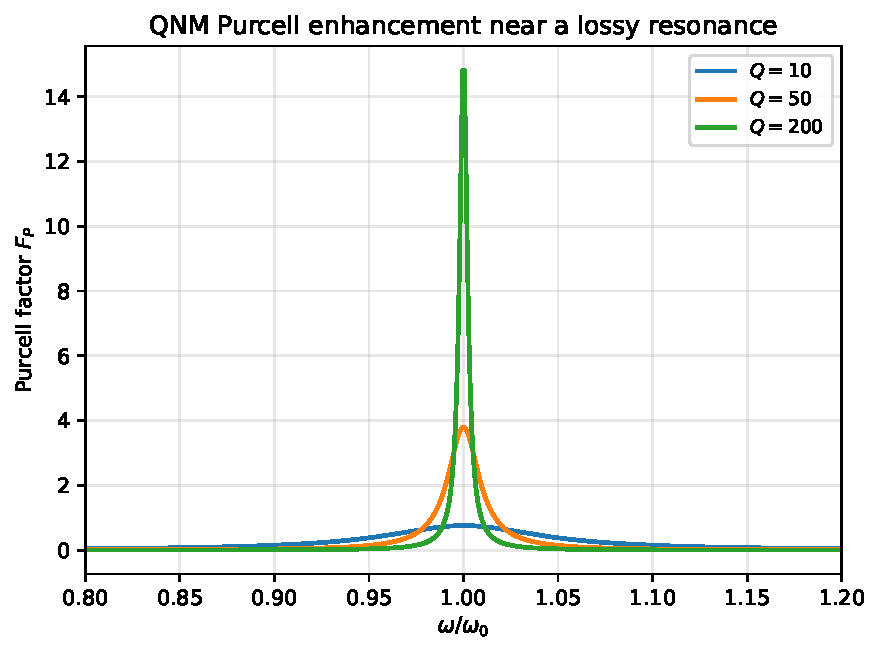
\includegraphics[width=0.6\linewidth]{figures/fig_f06_purcell_factor.pdf}
 \caption{Purcell enhancement factor $F_P(\omega)$ near a lossy
 optical resonance at $\omega_0$, computed from the QNM expansion for
 three quality factors $Q = 10$, $50$, and $200$. Higher $Q$ gives a
 taller and narrower Lorentzian peak, illustrating the trade-off
 between enhancement and bandwidth. In non-Hermitian systems, the
 Petermann factor introduces an additional correction
 (Section~\ref{sec:petermann}).}
 \label{fig:purcell-factor}
\end{figure}

\begin{takeaway}[The QNM Purcell factor]
The standard Purcell formula $F_P \propto \Qfac/V$ remains valid for open
cavities as a single-mode approximation, provided $V$ is understood as
the complex QNM mode volume and the observable rate is obtained from the
imaginary part of the Green tensor. In weakly lossy, isolated resonances
this often reduces to using $\Re\tilde{V}$ in the denominator. Using a
Hermitian, conjugated mode volume in place of the unconjugated QNM
normalization generally gives incorrect results for open or dissipative
cavities.
\end{takeaway}


%% ================================================================
\section{Perturbation theory for QNMs}
\label{sec:qnm-perturbation}

The biorthogonal framework provides a natural perturbation theory for
QNM eigenfrequencies. If the permittivity is perturbed by
$\delta\epsr(\rr)$ (e.g., by a nanoparticle binding event, a
temperature change, or a refractive-index modulation), the first-order
shift of the $n$-th QNM frequency is
\begin{equation}
 \delta\omtil_n = -\frac{\omtil_n}{2}
 \frac{\int \delta\epsr(\rr)\,\tilde{\EE}_n(\rr)\cdot\tilde{\EE}_n(\rr)\;\dd^3r}
 {\int \epsr(\rr)\,\tilde{\EE}_n(\rr)\cdot\tilde{\EE}_n(\rr)\;\dd^3r}.
 \label{eq:qnm-perturbation}
\end{equation}
This formula is the non-Hermitian analogue of the standard Rayleigh--Schr\"odinger
perturbation theory, with the unconjugated norm replacing the Hermitian
norm. Several features distinguish it from the Hermitian case:
\begin{itemize}
 \item The perturbation shift $\delta\omtil_n$ is complex: both the
 resonance frequency and the decay rate change simultaneously.
 \item The integrals involve $\tilde{\EE}_n \cdot \tilde{\EE}_n$
 (unconjugated), not $|\tilde{\EE}_n|^2$ (conjugated). For QNMs
 with large spatial divergence, these are very different.
 \item Near an exceptional point, where two QNMs coalesce, the
 denominator approaches zero and the perturbation theory breaks
 down---the response becomes $\propto\sqrt{\delta\epsr}$ rather than
 linear.
\end{itemize}

\paragraph{Example: nanoparticle sensing.}
Consider a dielectric nanoparticle of radius $a = 30\;$nm and
permittivity $\varepsilon_p = 2.25$ (silica) placed at the field maximum
of a photonic crystal cavity with $\omtil_0 = (1.22 - 0.015i) \times
10^{15}\;$rad/s ($\lambda \approx 1550\;$nm, $\Qfac \approx 40$). The
perturbation is $\delta\varepsilon = (\varepsilon_p - 1) = 1.25$ over
the nanoparticle volume $V_p = (4/3)\pi a^3 \approx 1.13 \times
10^{-22}\;$m$^3$. Using~\eqref{eq:qnm-perturbation} with a mode
volume $\tilde{V} \approx (0.8 - 0.2i)(\lambda/n)^3$ and
$\tilde{\EE}(\rr_0) \cdot \tilde{\EE}(\rr_0) \approx 1/\tilde{V}$
(from the normalization), the fractional frequency shift is
\begin{equation}
 \frac{\delta\omtil}{\omtil_0} \approx
 -\frac{\delta\varepsilon\,V_p}{2\,\varepsilon\,\tilde{V}}
 \approx -(1.4 - 0.3i) \times 10^{-4}.
 \label{eq:sensing-shift}
\end{equation}
The real part gives a resonance shift
$\delta\omega \approx -1.7 \times 10^{11}\;$rad/s ($\delta\lambda
\approx 0.22\;$nm), while the imaginary part gives a linewidth change
$\delta\gamma \approx 3.7 \times 10^{10}\;$rad/s. Both are
measurable in a standard transmission experiment. The key insight is
that the QNM perturbation theory predicts the linewidth shift as well
as the frequency shift, in contrast to Hermitian perturbation theory
which gives only the real frequency shift.


%% ================================================================
\section{Modal non-orthogonality and the Petermann factor}
\label{sec:petermann}

In a Hermitian system, the eigenmodes are orthogonal and the overlap
matrix $\langle\HH_m|\HH_n\rangle$ is diagonal. In a non-Hermitian
system, the QNMs are biorthogonal but generally not orthogonal under the
Hermitian inner product. This non-orthogonality has measurable physical
consequences.

The \emph{Petermann excess noise factor} $K_n$ for a laser mode
$\tilde{\EE}_n$ quantifies the degree of modal non-orthogonality:
\begin{equation}
 K_n = \frac{
 \langle\tilde{\EE}_n|\tilde{\EE}_n\rangle\,
 \langle\tilde{\EE}_n^{\mathrm{L}}|\tilde{\EE}_n^{\mathrm{L}}\rangle
 }{
 |\langle\tilde{\EE}_n^{\mathrm{L}}|\tilde{\EE}_n\rangle|^2
 } \ge 1.
 \label{eq:petermann}
\end{equation}
For an orthogonal (Hermitian) mode, $K_n = 1$. Near an exceptional
point, where two QNMs coalesce, $K_n$ diverges: the mode becomes
maximally non-orthogonal, and the laser linewidth is enhanced by a factor
$K_n$ above the Schawlow--Townes limit.

This connection between modal non-orthogonality, excess noise, and
exceptional points is one of the central links between the abstract
theory of non-Hermitian operators and measurable optical phenomena. It
will be revisited in Chapter~\ref{ch:exceptional-points}, where
exceptional-point sensing and noise limits are analyzed in detail.


%% ================================================================
\section{Completeness and limitations}
\label{sec:qnm-completeness}

\subsection{The completeness question}
\label{ssec:qnm-completeness-question}

The QNMs of an open system do not, by themselves, form a complete basis
in the mathematical sense~\cite{wu2024frontiers,opg2023dispersive,lasson2014roundtrip}. The full spectral decomposition includes the
continuous spectrum of radiation modes
(Section~\ref{sec:open-spectrum})~\cite{vial2014quasimodal}.

In the Green-tensor expansion~\eqref{eq:green-qnm}, the QNM sum captures
the \emph{pole} contribution to $\mathbf{G}(\omega)$. The remaining
contribution---the integral over the branch cut in the complex $\omega$
plane, which represents the continuous radiation spectrum---is missed.
This branch-cut contribution is typically small near a QNM resonance
(where the pole dominates) but can be significant far from resonance or
for broadband excitations.

\paragraph{The branch-cut integral.}
For a one-dimensional system, the Green function can be written
exactly as
\begin{equation}
 G(z, z'; \omega) = \sum_n \frac{\tilde{E}_n(z)\,\tilde{E}_n(z')}
 {2\omtil_n(\omega - \omtil_n)}
 + \frac{1}{2\pi i}\int_{\mathcal{B}}
 \frac{g(z, z'; \omega')}{\omega - \omega'}\;\dd\omega',
 \label{eq:green-complete}
\end{equation}
where the first sum is over QNM poles and the second integral is over
the branch cut $\mathcal{B}$ in the complex $\omega$ plane, which runs
along the negative imaginary axis for outgoing-wave boundary conditions.
The branch-cut integrand $g(z, z'; \omega')$ represents the contribution
of radiation modes that form a continuum rather than discrete poles.

For a high-$\Qfac$ resonator driven near a single QNM, the pole term
dominates by a factor of $\sim \Qfac$, and the branch-cut contribution
can be neglected. For broadband excitation or for frequencies between
well-separated QNMs, the branch-cut contribution provides a smooth
background that fills in the spectral gaps between resonances. The
Riesz-projection method of Wu and Lalanne~\cite{wu2026rigorous}
handles this background systematically by computing both the pole
residues and the background response from a single set of complex-frequency
simulations.

\subsection{When is a QNM expansion sufficient?}
\label{ssec:qnm-sufficiency}

The accuracy of a truncated QNM expansion depends on:
\begin{enumerate}
 \item the $\Qfac$ of the relevant modes (higher $\Qfac$ means narrower
 resonances and better QNM dominance);
 \item the spectral distance from other resonances (isolated resonances
 are better described);
 \item the spatial extent of the source or field of interest (sources
 far from the resonator couple more to radiation modes);
 \item the number of modes retained (keeping more QNMs captures
 more of the spectral response, but the branch cut is always
 missed).
\end{enumerate}

For most nanophotonic applications---Purcell enhancement, SERS,
nonlinear harmonic generation in and near a single resonator---a few-QNM
expansion is sufficient. For broadband scattering problems, a background
correction or a Riesz-projection approach is needed to capture the
non-resonant contribution~\cite{wu2026rigorous}.

\subsection{Relation to coupled-mode theory}
\label{ssec:qnm-cmt-bridge}

A QNM expansion truncated to a small number of modes is, in effect, a
\emph{coupled-mode model}: the field is represented as a superposition
of a few resonant modes, each with a complex frequency, and the dynamics
are governed by a finite-dimensional non-Hermitian matrix. The
difference from phenomenological coupled-mode theory is that the QNM
expansion is \emph{derived from Maxwell's equations} with controlled
approximations, and the coupling coefficients are determined by the
mode overlaps, not by fitting.

This connection between QNMs and effective Hamiltonians is the subject
of Chapter~\ref{ch:maxwell-coupled-modes}, where the coupled-mode
formalism is developed explicitly from the Maxwell operator.
